\documentclass{sig-alternate-2013}

\setlength{\paperheight}{11in}
\setlength{\paperwidth}{8.5in}

\usepackage[pass]{geometry}
\usepackage[nocompress]{cite}
\usepackage[utf8]{inputenc}
\usepackage{hyperref}
%% url
\usepackage{url}
%% maths
%%\usepackage[cmex10]{amsmath}
%%\usepackage{amsfonts}
%%\usepackage{amssymb}
%%\usepackage{amsthm}
\usepackage{mathtools}
%% algorithms
\usepackage{algorithm}
\usepackage{algorithmicx}
\usepackage{algpseudocode}
%% images
\usepackage{graphicx}
%% inparaenum
\usepackage[defblank]{paralist}
%% tables
\usepackage{booktabs}
\usepackage{multirow}
%% figures
\usepackage{subfig}
\usepackage{tikz}
\usetikzlibrary{decorations.pathreplacing,plotmarks,shapes,matrix}
%% transform eps in pdf crossplateform
\usepackage{epstopdf}
\usepackage{epsfig}
%% hyphenation
\usepackage{hyphenat}
\hyphenation{brow-sers brow-ser}

\newcommand{\TODO}[1]{\textcolor{red}{#1}}
\newcommand{\REF}[0]{\textcolor{purple}{REF}}


\usepackage{xspace}
\newcommand{\SCAMP}[0]{\textsc{Scamp}\xspace}
\newcommand{\CYCLON}[0]{\textsc{Cyclon}\xspace}
\newcommand{\SPRAY}[0]{\textsc{Spray}\xspace}
\newcommand{\LSEQ}[0]{\textsc{LSeq}\xspace}
\newcommand{\CRATE}[0]{\textsc{Crate}\xspace}
\newcommand{\PEERSIM}[0]{\textsc{PeerSim}\xspace}

\setlength{\belowcaptionskip}{-10pt} %% reduce spacing below figures

%paralist
\renewcommand*\descriptionlabel[1]{%
\scshape #1}
\renewcommand\paradescriptionlabel[1]{%
\scshape #1}

%%%%%%%%%%%%%%%%%%%%%%%%%%%%%%%%%%%%%%%%%%%%%%%%%%%%%%%%%%%%%%%%%%%%%%%%%%%%%%%
%%%%%%%%%%%%%%%%%%%%%%%%%%%%%%%%%%%%%%%%%%%%%%%%%%%%%%%%%%%%%%%%%%%%%%%%%%%%%%%
%%%%%%%%%%%%%%%%%%%%%%%%%%%%%%%%%%%%%%%%%%%%%%%%%%%%%%%%%%%%%%%%%%%%%%%%%%%%%%%

%% remove the extra dot at the end of the DOI
\toappear{\the\boilerplate\par
{\confname{\the\conf}} \the\confinfo\par \the\copyrightetc}


\permission{Copyright is held by the International World Wide Web Conference
  Committee (IW3C2). IW3C2 reserves the right to provide a hyperlink to the
  author's site if the Material is used in electronic media.}
\conferenceinfo{WWW'16 Companion,}{April 11--15, 2016, Montr\'eal, Qu\'ebec,
  Canada.}
\copyrightetc{ACM \the\acmcopyr}
\crdata{978-1-4503-4144-8/16/04. \\
DOI: http://dx.doi.org/10.1145/2872518.2890539}

\clubpenalty=10000 
\widowpenalty = 10000

\begin{document}


\title{CRATE: Writing Stories Together with our Browsers}

\numberofauthors{3}
\author{
\alignauthor
Brice N{\'e}delec\\
\affaddr{Universit{\'e} de Nantes, LINA}\\
\affaddr{2 rue de la Houssini{\`e}re}\\
\affaddr{Nantes, France}%\\
%\email{\mbox{brice.nedelec{@}univ-nantes.fr}}
\alignauthor
Pascal Molli\\
\affaddr{Universit{\'e} de Nantes, LINA}\\
\affaddr{2 rue de la Houssini{\`e}re}\\
\affaddr{Nantes, France}\\
\email{\mbox{first.last{@}univ-nantes.fr}}
\alignauthor
Achour Mostefaoui\\
\affaddr{Universit{\'e} de Nantes, LINA}\\
\affaddr{2 rue de la Houssini{\`e}re}\\
\affaddr{Nantes, France}%\\
%\email{\mbox{achour.mostefaoui{@}univ-nantes.fr}}
}
\date{}

\maketitle

\begin{abstract}
  Real-time collaborative editors are common tools to distribute work across
  space, time, and organizations. Unfortunately, mainstream editors such as
  Google Docs rely on central servers and raises privacy and scalability issues.
  \CRATE is a real-time decentralized collaborative editor that runs directly in
  web browsers thanks to WebRTC. Compared to state-of-the-art, \CRATE is the
  first real-time editor that only requires browsers to support collaborative
  editing and to transparently handle from small to large groups of
  users. Consequently, \CRATE can also be used in massive online lectures, TV
  shows or large conferences to allow users to share their notes. \CRATE
  properties rely on two scientific results:
  \begin{inparaenum}[(i)]
  \item a replicated sequence structure with sub-linear upper bound on space
    complexity; this prevents the editor from running costly distributed garbage
    collectors,
  \item an adaptive peer sampling protocol; this prevent the editor from
    oversizing routing tables, hence from letting small networks pay the price
    of large networks.
  \end{inparaenum}
  This paper describes \CRATE, its properties and its usage.
\end{abstract}

\keywords{Collaborative editor, decentralized, real-time}

%%% Local Variables:
%%% mode: latex
%%% TeX-master: "../paper"
%%% End:



\section{Introduction}
\label{sec:introduction}

Real-time collaborative editors allow authors to simultaneously write shared
documents. Trending editors such as Google Docs rely on
central servers. They raise privacy issues since service providers take
advantage of their mediating position to observe all users and documents. They
also raise scalability issues, for they require a server to support an editing
session, so handling many editing sessions requires many resources. Also
managing large editing sessions puts a lot of pressure on the server which may
become overloaded.

%% managing many participants in one editing session is costly and may overload the
%% server.

\CRATE is a distributed and decentralized \textsc{c}ollabo\textsc{rat}ive
\textsc{e}ditor providing scalable real-time editing capabilities directly
within web browsers. Compared to state-of-the-art, \CRATE is the first real-time
editor that only requires browsers in order to support collaborative editing and
to transparently handle from small to large groups of users.

Suppose massive online lecture platforms allow students to share their
notes. Many lectures run in parallel involving various number of students, i.e.,
from few to thousands. Also, even during the editing session the audience is subject
to significant changes in size, going from thousands to hundreds. Finally, the
resulting document size is hardly predictable, for it depends of the number and
zealous of involved students.
%% even during one editing session, the number of participants can change
%% significantly, from thousands to few hundreds. The size of document
%% produced by users is also hard to predict: it can vary from few pages
%% to hundreds of pages. 

\CRATE handles these situations by combining different algorithms to achieve an
acceptable trade-off between space, time and communication complexities. In
laboratory, we observed this trade-off on configurations involving up till 600
browsers. In this paper, we describe the usage, the architecture and the
properties of \CRATE. Also we propose a live experiment to WWW2016 participants
aiming to confirm laboratory experiments about \CRATE.

Section~\ref{sec:usage} depicts the usage of \CRATE.
Section~\ref{sec:architecture} details the overall architecture of \CRATE along
with its basic functioning. Section~\ref{sec:network} shows the way to build
decentralized networks directly in browsers.  Section~\ref{sec:structure}
describes the distributed data structure that represents the document.
Section~\ref{sec:live} shows our laboratory result and describes the live
experiment setup. Section~\ref{sec:conclusion} concludes.


%%% Local Variables:
%%% mode: latex
%%% TeX-master: "../paper"
%%% End:


\section{Usage}

\CRATE is a real-time collaborative editor running in web browsers. As a web
application, it is hosted on a web server at
\emph{\url{http://chat-wane.github.io/CRATE/}}. Hence, users simply navigate to
the web page with their web browser\footnote{A small restriction being that it
  must support WebRTC.}.

A user creates a document. At the time, the document is only local and no one
can read or modify it apart from its creator. When the user is ready to share
its content with collaborators of his, he simply copy--pastes a uniform resource
locator (URL) to them. Once the collaborators open the link, it automatically
connects them to the editing session of the creator. It retrieves the shared
document and they can start the real-time collaborative editing.

\section{Architecture}
\label{sec:architecture}

\begin{figure}
  \centering
  \begin{tikzpicture}[scale=0.9]

\newcommand\X{25pt}
\newcommand\Y{20pt}

\newcommand\LIGHTERGRAY{base3}
\newcommand\LIGHTGRAY{base2}
\newcommand\MEDIUMGRAY{yellow}

\small
%% communication
\draw[rounded corners=2mm, color=\MEDIUMGRAY, fill=\LIGHTERGRAY](0pt, 0pt)+(-4*\X,-\Y)rectangle+(4*\X,\Y);
\draw(4*\X, \Y)node[anchor=north east]{\textbf{communication}};

\draw[fill=\LIGHTERGRAY](-2*\X, -0.25*\Y)
node{broadcast}+(-0.75*\X,-0.5*\Y)rectangle+(0.75*\X,0.5*\Y);
\draw[fill=\LIGHTERGRAY, very thick]( 0*\X, 0.25*\Y)
node[align=center]{membership\\\SPRAY}+(-0.85*\X,-0.5*\Y)rectangle+(0.85*\X,0.5*\Y);
%%\draw[fill=white]( 2*\X, -0.25*\Y)
%% node{unicast}+(-0.75*\X,-0.5*\Y)rectangle+(0.75*\X,0.5*\Y);

\draw[<-](-0.85*\X, 0.25*\Y)--(-1.25*\X, -0.25*\Y);
%% \draw[<-](0.85*\X, 0.25*\Y)--(1.25*\X, -0.25*\Y);

%% causality
\draw[rounded corners=2mm, color=\MEDIUMGRAY, fill=\LIGHTGRAY](0pt, -2*\Y)+(-4*\X,-\Y)rectangle+(4*\X,\Y);
\draw(4*\X, -\Y)node[anchor=north east]{\textbf{causality}};

\draw[fill=\LIGHTGRAY](-2*\X, -2*\Y)
node[align=center]{version vector\\with\\exceptions}
+(-1.0*\X,-0.6*\Y)rectangle+(1.0*\X,0.6*\Y);
\scriptsize
\draw[->, thick](-1.5*\X, -0.75*\Y) -- node[anchor=west]{receive}
(-1.5*\X, -1.4*\Y);
\draw[<-, thick](-2.5*\X, -0.75*\Y) -- node[anchor=east]{send}
(-2.5*\X, -1.4*\Y);
\small
%% \draw[<->]( 2*\X, -0.75*\Y)--( 1*\X, -2.5*\Y);

%% sequence structure
\draw[rounded corners=2mm, color=\MEDIUMGRAY, fill=\LIGHTERGRAY](0pt, -4*\Y)+(-4*\X,-\Y)rectangle+(4*\X,\Y);
\draw(4*\X, -3*\Y)node[anchor=north east, align=right]
{\textbf{sequence}\\\textbf{structure}};

%% \draw[fill=white, shading=axis,top color=\LIGHTGRAY, bottom color=white, shading angle=0](1*\X, -3*\Y)
%% node{anti-entropy}+(-0.95*\X,-0.5*\Y) rectangle +(0.95 *\X, 0.5*\Y);
\draw[fill=\LIGHTERGRAY, very thick](-2*\X, -4*\Y)
node{\LSEQ}+(-0.75*\X,-0.5*\Y) rectangle +(0.75 *\X, 0.5*\Y);

%\draw[->] (0.05*\X, -2.75*\Y)--(-1*\X,-2*\Y);
%\draw[->] (0.05*\X, -3.25*\Y)--(-1.25*\X,-4*\Y);
\scriptsize
\draw[<-, thick] (-1.5*\X, -3.5*\Y)--node[anchor=west]{deliver}(-1.5*\X, -2.6*\Y);
\draw[->, thick] (-2.5*\X, -3.5*\Y)--node[anchor=east]{decorate}(-2.5*\X, -2.6*\Y);
\small
%% gui
\draw[rounded corners=2mm, color=\MEDIUMGRAY, fill=\LIGHTGRAY](0pt, -6*\Y)+(-4*\X,-\Y)rectangle+(4*\X,\Y);
\draw(4*\X, -5*\Y)node[anchor=north east, align=right]
{\textbf{graphical}\\\textbf{user}\\\textbf{interface}};
\draw[fill=\LIGHTGRAY](0pt,-6*\Y)
node{web editor}+(-0.85*\X,-0.5*\Y) rectangle +(0.85 *\X, 0.5*\Y);

%%\draw[<->] (-2*\X, -4.5*\Y) -- (0*\X, -5.5*\Y);
\scriptsize
\draw[->, thick] (-1.80*\X, -4.5*\Y)--node[anchor=west]{notify}(-0.85*\X, -5.75*\Y);
\draw[<-, thick] (-2.20*\X, -4.5*\Y)--node[anchor=east]{update}(-0.85*\X, -6.25*\Y);
\small
\end{tikzpicture}
  \caption{\label{fig:architecture} Four layers architecture of \CRATE.}
\end{figure}

\CRATE is based on the optimistic replication
scheme~\cite{saito2005optimistic}. Thus, each editor replicates the
document locally and directly performs operations on it. Next, changes
are spread to all other participants. When the same set of operations
are applied by editors, the replicates converge to an equivalent state
allowing users to read the same document.  This property is called
\emph{strong eventual consistency}~\cite{bailis2013eventual}.

\CRATE uses a Conflict-free Replicated Data Type (CRDT) for sequences to ensure
strong eventual consistency on the
document~\cite{shapiro2011comprehensive}. They ensure consistency at the price
of a unique identifier attached to each element of the sequence. Recently,
\LSEQ~\cite{nedelec2013lseq} proposed a strategy to bound the space complexity
of these identifiers to $\mathcal{O}(\log(d)^2)$ where $d$ is the document
size. This result avoids to run costly distributed garbage-collection-like
mechanisms to maintain the efficiency of the editor.

Eventual consistency requires that all operations are received by all editing
session members.  \CRATE builds an editing session using
\SPRAY~\cite{nedelec2015spray}, a random peer sampling
protocol~\cite{jelasity2007gossip} (RPS) built on top of WebRTC. A peer sampling
protocol provides each network member with a partial view of the network
significantly smaller compared to this latter. Maintaining this partial view
random ensures the connectivity of the network. Unlike prior RPS, \SPRAY allows
adapting the partial view sizes to the editing session size without
measuring its number of participants. Since the propagation protocol of
messages~\cite{birman1999bimodal} extensively uses these tables, the network
traffic inherits from this scalability. Consequently, \CRATE adapts its
operation to the need of the editing session size.


The distributed and decentralized \textsc{c}ollabo\textsc{rat}ive
\textsc{e}ditor \CRATE developed in web languages only: HTML, CSS, and mostly
JavaScript. As shown in Figure~\ref{fig:architecture}, \CRATE comprises four
layers:
\begin{asparadesc}
\item [\textbf{The graphical user interface}] that renders the document to the users
  (cf. Figure~\ref{img:screenshot}). Each local update is immediately applied to
  the document view for real-time sake. Then, the update is applied to the
  replicated data type;
\item [\textbf{The sequence structure layer}] that represents the local document
  (cf. §\ref{sec:structure}). It is in charge of providing the metadata
  necessary to order each character identically anywhere;
\item [\textbf{The causality layer}] that tracks semantic causality between operations,
  e.g., the removal of a character cannot precede its insertion;
\item [\textbf{The network layer}] that
  \begin{inparaenum}[(i)]
  \item builds a network of browsers for each editing session and
  \item uses it to propagate the updates to all collaborators
    (cf. §\ref{sec:network}).
  \end{inparaenum}
\end{asparadesc}



%%% Local Variables:
%%% mode: latex
%%% TeX-master: "../paper"
%%% End:


\section{Network of browsers}
\label{sec:network}

\begin{figure}
  \centering
  
\begin{tikzpicture}[scale=1]

  \newcommand\X{25pt}
  \newcommand\Y{-25pt}

  \draw[->] (\X, 0)--(\X, 5+3*\Y); %% p1 p6
  \draw[->] (-5+2*\X, 0)--(5+\X, 0); %% p2 p1
  \draw[->] (2*\X, 0) -- (-5+3*\X, \Y); %% p2 p3
  \draw[->] (2*\X, 0) -- (-5+3*\X, 2*\Y); %% p2 p4
  \draw[->] (3*\X, 5+\Y) -- ( 5+2*\X, 0); %% p3 p2
  \draw[->] (3*\X, \Y) -- (5pt, 2*\Y); %% p3 p7
  \draw[->] (3*\X, \Y) -- (2*\X, 5+3*\Y); %% p3 p5
  \draw[->] (3*\X, 2*\Y) -- (5pt, 2*\Y); %% p4 p7
  \draw[->] (3*\X, 2*\Y) -- (5pt, \Y); %% p4 p8
  \draw[->] (2*\X, 3*\Y) -- (\X, -5pt); %% p5 p1
  \draw[->] (5+2*\X, 3*\Y) -- (3*\X, -5+ 2*\Y); %% p5 p4
  \draw[->] (-5+\X, 3*\Y) -- (0pt, -5+2*\Y); %% p6 p7
  \draw[->] (0pt, 2*\Y) -- (-5+3*\X, \Y); %% p7 p3
  \draw[->] (0pt, 2*\Y) -- (\X, -5pt); %% p7 p1
  \draw[->] (0pt, \Y) -- (2*\X, -5pt); %% p8 p2
  \draw[->] (0pt, \Y) -- (\X, 5+3*\Y); %% p8 p6
  \draw[->] (0pt, \Y) -- (-5+3*\X, \Y); %% p8 p3
  
  \scriptsize
  \draw[fill=base3] (-2*\X, 1.5*\Y) node{$e_9$} +(-5pt,-5pt) rectangle +(5pt,5pt);
  \draw[<->, densely dashed, color=blue, thick] (-2*\X, 5+1.5*\Y) -- node[anchor=east]{join \ } (-2*\X, -5pt);

  \draw[fill=base3] (-2*\X, 0) node{$mediator_1$} +(-20pt, -5pt)rectangle+(20pt, 5pt);
  \draw[<->, densely dashed, color=red, thick] (20-2*\X, 0) -- node[anchor=south]{share} (-5+\X, 0);
  \draw[<->, densely dashed, color=red, thick] (20-2*\X, -5pt) -- (-5pt, \Y);
  
  \draw[fill=base3] (-2*\X, 3*\Y) node{$mediator_2$} +(-20pt, -5pt)rectangle+(20pt, 5pt);
  \draw[<->, densely dashed, color=red, thick] (20-2*\X, 3*\Y) -- (-5+\X, 3*\Y);
  \draw[<->, densely dashed, color=red, thick] (20-2*\X, 5+3*\Y) -- (-5pt, 2*\Y);

  \draw[fill=base3] (\X, 0)node{$e_1$}+(-5pt, -5pt)rectangle+(5pt, 5pt);
  \draw[fill=base3] (2*\X, 0)node{$e_2$}+(-5pt, -5pt)rectangle+(5pt, 5pt);
  \draw[fill=base3] (3*\X, \Y)node{$e_3$}+(-5pt, -5pt)rectangle+(5pt, 5pt);
  \draw[fill=base3] (3*\X, 2*\Y)node{$e_4$}+(-5pt, -5pt)rectangle+(5pt, 5pt);
  \draw[fill=base3] (2*\X, 3*\Y)node{$e_5$}+(-5pt, -5pt)rectangle+(5pt, 5pt);
  \draw[fill=base3] (1*\X, 3*\Y)node{$e_6$}+(-5pt, -5pt)rectangle+(5pt, 5pt);
  \draw[fill=base3] (0 , 2*\Y)node{$e_7$}+(-5pt, -5pt)rectangle+(5pt, 5pt);
%  \draw[fill=base3] (0 , \Y)+(-55pt, -10pt)rectangle+(5pt, 10pt);
  \draw[fill=base3](0,\Y) node{$e_8$}+(-5pt, -5pt)rectangle+(5pt, 5pt);

\end{tikzpicture}
  \caption{Example of a small network built by \SPRAY. Each editor $e$ can
    communicate with a small partial view of the network. For instance, Editor
    $e_8$'s partial view comprises $e_2$, $e_3$ and $e_6$. In addition, $e_1$
    and $e_8$ grant a public access to the editing session through
    $mediator_1$. Editor $e_9$ is joining.}
  \label{fig:spray}
\end{figure}


\CRATE uses \SPRAY to build a network of browsers thanks to WebRTC. The latter
is a recent technology that allows establishing browser-to-browser channels of
communication. Its connection establishment protocol imposes a round-trip of
messages. Thus, if an editor $e_1$ wants to connect to another editor $e_2$, it
needs to send a message to $e_2$ and to acknowledge its response. While the
first of such connection must use a mediator (e.g. mail, dedicated server etc.),
once established, the network can assume the position of mediator and start
working autonomously.

Random peer sampling protocols provide each editor with a local neighborhood
table. These tables allow communicating to a subset of peers (here
editors). Messages can travel from neighbor to neighbor to reach any editor in a
scalable manner.

%% Web browsers exist in most of current devices. \TODO{Moar.}

%% \SPRAY is an adaptive random peer sampling protocol which provides each editor
%% with a neighborhood table the size of which grows and shrinks following the
%% global network size, yet without any global knowledge. 

\SPRAY's lifecycle at each editor comprises three steps that aim to provide and
maintain logarithmically scaling neighborhood tables compared to the editing
session size:
\begin{asparadesc}
\item [\textbf{The joining:}] the editor wants to join the editing session. It
  contacts an editor inside the network and waits for its answer to establish
  the very first WebRTC connection between them. Using this connection, the
  joining editor asks to its contact editor to operate as mediator to advertise
  its presence to the contact's neighbors. Each of these neighbors connects to
  the joining peer. Since the number of neighbor is supposed logarithmic, the
  number of connections in the network grows by $\log(N)+1$ where $\log(N)$ is
  the natural logarithm of the network size $N$. Following such growth, the
  number of connections globally is $N.\log(N)$.
\item [\textbf{The shuffling:}] each editor regularly initiates a table
  shuffling with the oldest of its neighbors. The initiator serves as mediator
  between half of its neighborhood chosen at random and the oldest neighbor. In
  response, the oldest neighbor does the same. As a result, they roughly have an
  identical neighborhood size which tackles the load-balancing problem that may
  rise from the joining part of the protocol. It is worth noting that the number
  of connection remains constant. In addition, the references in neighborhood
  tables are randomly distributed. The network converges in exponential time
  toward a topology exposing properties similar to those of random
  graphs~\cite{erdos1959random} (cf. Figure~\ref{fig:spray}).
\item [\textbf{The leaving:}] the editor can leave the network without giving
  notice, i.e., equivalent to a crash. Nevertheless, its removal from the system
  must lead to a decrease of $\log(N)+1$ connections while currently it
  represents $\log(N)$ connections from its neighborhood tables, and $\log(N)$
  connections from other editors' neighborhood tables pointing to it. The
  adjusting falls under the responsibility of these other editors. For this
  purpose, they detect the departure of a neighbor when they try to initiate a
  shuffle with it. Since such detection presumably happen $\log(N)$ times, they
  all duplicate one of their neighbors except for one; the probability being
  processed using their own neighborhood table size. 
\end{asparadesc}

Such random peer sampling protocol constitutes the ground of various protocols
such as topology managements. \CRATE uses it to disseminate all operations of
the replicated sequence to all collaborators in a scalable manner. Referred as
epidemic dissemination, rumor mongering, or gossiping, the protocol is a
two-step operation:
\begin{inparaenum}[(i)]
\item Each operation performed on the local document replica leads to the
  creation of a message. The latter is sent to all the neighborhood provided by
  \SPRAY.
\item Each editor receiving such broadcast message transmits it again to its
  neighborhood.
\end{inparaenum}
Thus, messages transitively reach all collaborators very efficiently.  This
dissemination protocol inherits from \SPRAY's adaptiveness. Hence, traffic
follows the editing session size.

Prior approaches generally oversize the partial views to handle largest groups
of users. Unfortunately, smaller groups suffer from such \emph{a priori}
dimensioning. Since \SPRAY automatically adjusts neighborhood table sizes, it
equally handles from smallest to largest groups.

%%% Local Variables:
%%% mode: latex
%%% TeX-master: "../paper"
%%% End:


\section{Replicated document}
\label{sec:structure}

To provide eventually consistent replicas, \CRATE uses a conflict-free
replicated data type for sequences~\cite{shapiro2011comprehensive}. Such
sequence type avoids the difficult and error-prone task of solving conflicts by
the mean of commutative operations. Thus, the sequence type provides two basic
operations: the insertion and removal of an element. If two users perform
concurrently some operations at an identical position in the sequence, the
latter will still converge to an equivalent state.

Commutativity comes at the price of additional metadata attached to each
element of the sequence. These metadata referred to as identifier are unique,
immutable, and of variable size at generation. When a character is inserted, the
sequence type generates an identifier which is a list
$[\ell_1.\ell_2\ldots \ell_k]$ where $k$ is the identifier depth and Element
$\ell_i$ comprises a path $p_i$, a globally unique site identifier $s_i$, a
monotonic local counter $c_i$.

A lexicographic total order amongst these identifiers allows retrieving the
sequence:
\begin{align*}
  \ell_i < \ell_j \iff & (p_i < p_j) \vee \\
                       & ((p_i = p_j) \wedge (s_i<s_j)) \vee \\
                       & ((p_i = p_j) \wedge (s_i = s_j) \wedge (c_i < c_j)) \\
  \ell_i = \ell_j \iff & \neg (\ell_i < \ell_j) \wedge \neg (\ell_j < \ell_i) \\
  i_i < i_j \iff & \exists (m > 0)(\forall n < m) (\ell^i_n = \ell^j_n) \wedge (\ell^i_m < \ell^j_m) \\
  i_i = i_j \iff & (\forall m) \ell^i_n = \ell^j_n
\end{align*}

The first two equivalences define an ordering between elements of the list
composing the identifiers. The last two equivalences use these to define a
global total order amongst identifiers, hence, ordering characters of the
document. While the third equivalence is mostly used to locate the proper
inserting position, the fourth equivalence is necessary for removals.  Paths of
identifiers constitute the most discriminant part of identifiers, hence the most
important part.

\CRATE uses \LSEQ to generate the paths of identifiers. The paths are series of
integers $[p_1.p_2\ldots p_k]$ where each path is chosen among a set twice as
large as its preceiding path. For instance, if $p_1$ is chosen among
$\{0..2^8\}$ then $p_2$ is chosen among $\{0..2^9\}$ etc.  When the document
grows, the depth of identifiers is expected to grow. Therefore, increasing the
size of sets over depths decreases the growth in depth. In turn, \LSEQ allocates
identifiers polylogarithmically upper-bounded compared to the number of
insertions in the sequence, and without \emph{a priori} knowledge of the series
of updates.

Keeping the size under such a sub-linear bound avoids the need of an unafordable
distributed garbage-collecting-like mechanism.

%%% Local Variables:
%%% mode: latex
%%% TeX-master: "../paper"
%%% End:


\section{Experiments}
\label{sec:live}

\begin{figure}
  \centering
  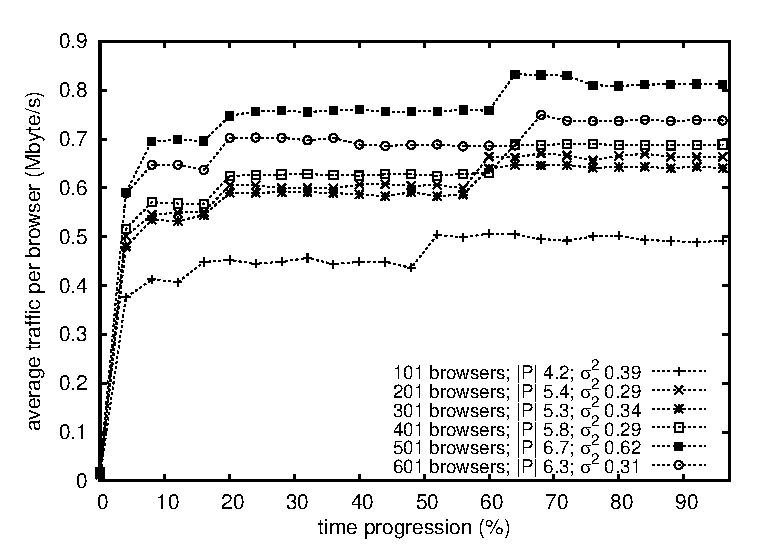
\includegraphics[width=0.49\textwidth]{img/traffic.eps}
  \caption{\label{fig:traffic}Average traffic per second.}
\end{figure}

In laboratory, we tested \CRATE on the Grid'5000 testbed with configurations
involving up till 600 browsers. Figure~\ref{fig:traffic} shows the traffic
generated at each member by intensive editing sessions. Overall, the artificial
authors insert 100 characters per second during 7 hours. The documents reach
millions of characters. Figure~\ref{fig:traffic} shows the combined effects of
\SPRAY and \LSEQ. Indeed, we observe that the traffic logarithmically scales to
the editing session size thanks to \SPRAY. The members of the smallest editing
session (101 browsers) are less traffic intensive than ones of the largest group
(601 browsers).  But the messages transiting the network are important too. The
growth of each plot corresponds to the identifiers size generated by
\LSEQ. Since the document size grows, the identifiers grow, but their growth
slows over insertions.


% \begin{figure*}
%   \centering
%   \subfloat[Figure A][\label{fig:liveA} Setup of the live
%   experiment. People start joining through a mediator server connected to our
%   replica. It incrementally builds an editing session with browsers
%   (cf. figure~\ref{fig:liveB}).]{
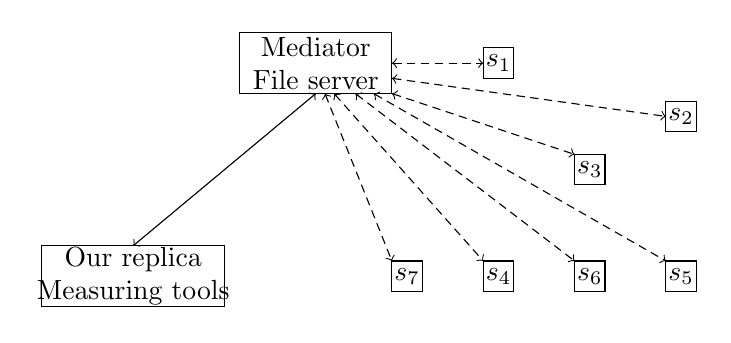
\begin{tikzpicture}[scale=1.1]
  
  \newcommand\X{30pt};
  \newcommand\Y{35pt};

  \draw[fill=white](0*\X, 0*\Y) node[align=center]{Mediator\\File server} +(-25pt,-10pt) rectangle +(25pt,10pt);
  \draw[fill=white](-2*\X, -2*\Y) node[align=center]{Our replica\\Measuring tools} +(-30pt,-10pt) rectangle +(30pt,10pt);

  \draw[fill=white](2*\X, -0*\Y)node{$s_1$} +(-5pt,-5pt) rectangle +(5pt,5pt);
  \draw[fill=white](4*\X, -0.5*\Y)node{$s_2$}  +(-5pt,-5pt) rectangle +(5pt,5pt);
  \draw[fill=white](3*\X, -1*\Y)node{$s_3$}  +(-5pt,-5pt) rectangle +(5pt,5pt);
  \draw[fill=white](2*\X, -2*\Y)node{$s_4$}  +(-5pt,-5pt) rectangle +(5pt,5pt);
  \draw[fill=white](4*\X, -2*\Y)node{$s_5$}  +(-5pt,-5pt) rectangle +(5pt,5pt);
  \draw[fill=white](3*\X, -2*\Y)node{$s_6$}  +(-5pt,-5pt) rectangle +(5pt,5pt);
  \draw[fill=white](1*\X, -2*\Y)node{$s_7$}  +(-5pt,-5pt) rectangle +(5pt,5pt);


  \draw[<->](0*\X, -10+0*\Y) -- (-2*\X, -2*\Y+10);
  \draw[<->, densely dashed] (0*\X+25,0*\Y) -- (2*\X-5, 0*\Y);
  
  \draw[<->, densely dashed] (0*\X+25,0*\Y-5) -- (4*\X-5, -0.5*\Y);
  \draw[<->, densely dashed] (0*\X+25,0*\Y-10) -- (3*\X-5, -1*\Y+5);
  \draw[<->, densely dashed] (0*\X+19,0*\Y-10) -- (4*\X-5, -2*\Y+5);
  \draw[<->, densely dashed] (0*\X+13,0*\Y-10) -- (3*\X-5, -2*\Y+5);
  \draw[<->, densely dashed] (0*\X+6,0*\Y-10) -- (2*\X-5, -2*\Y+5);
  \draw[<->, densely dashed] (0*\X+3,0*\Y-10) -- (1*\X-5, -2*\Y+5);

\end{tikzpicture}}
%   \hspace{10pt}
%   \subfloat[Figure B][\label{fig:liveB} Once connected, the editing session is
%   autonomous. The number of connections reflects the network size. Neigbhorhoods
%   are randomly filled and change over time.]{
\begin{tikzpicture}[scale=1]

  \newcommand\X{25pt}
  \newcommand\Y{-25pt}

  \draw[->] (\X, 0)--(\X, 5+3*\Y); %% p1 p6
  \draw[->] (-5+2*\X, 0)--(5+\X, 0); %% p2 p1
  \draw[->] (2*\X, 0) -- (-5+3*\X, \Y); %% p2 p3
  \draw[->] (2*\X, 0) -- (-5+3*\X, 2*\Y); %% p2 p4
  \draw[->] (3*\X, 5+\Y) -- ( 5+2*\X, 0); %% p3 p2
  \draw[->] (3*\X, \Y) -- (5pt, 2*\Y); %% p3 p7
  \draw[->] (3*\X, \Y) -- (2*\X, 5+3*\Y); %% p3 p5
  \draw[->] (3*\X, 2*\Y) -- (5pt, 2*\Y); %% p4 p7
  \draw[->] (3*\X, 2*\Y) -- (5pt, \Y); %% p4 p8
  \draw[->] (2*\X, 3*\Y) -- (\X, -5pt); %% p5 p1
  \draw[->] (5+2*\X, 3*\Y) -- (3*\X, -5+ 2*\Y); %% p5 p4
  \draw[->] (-5+\X, 3*\Y) -- (0pt, -5+2*\Y); %% p6 p7
  \draw[->] (0pt, 2*\Y) -- (-5+3*\X, \Y); %% p7 p3
  \draw[->] (0pt, 2*\Y) -- (\X, -5pt); %% p7 p1
  \draw[->] (0pt, \Y) -- (2*\X, -5pt); %% p8 p2
  \draw[->] (0pt, \Y) -- (\X, 5+3*\Y); %% p8 p6
  \draw[->] (0pt, \Y) -- (-5+3*\X, \Y); %% p8 p3
  
  \scriptsize
  \draw[fill=base3] (-2*\X, 1.5*\Y) node{$e_9$} +(-5pt,-5pt) rectangle +(5pt,5pt);
  \draw[<->, densely dashed, color=blue, thick] (-2*\X, 5+1.5*\Y) -- node[anchor=east]{join \ } (-2*\X, -5pt);

  \draw[fill=base3] (-2*\X, 0) node{$mediator_1$} +(-20pt, -5pt)rectangle+(20pt, 5pt);
  \draw[<->, densely dashed, color=red, thick] (20-2*\X, 0) -- node[anchor=south]{share} (-5+\X, 0);
  \draw[<->, densely dashed, color=red, thick] (20-2*\X, -5pt) -- (-5pt, \Y);
  
  \draw[fill=base3] (-2*\X, 3*\Y) node{$mediator_2$} +(-20pt, -5pt)rectangle+(20pt, 5pt);
  \draw[<->, densely dashed, color=red, thick] (20-2*\X, 3*\Y) -- (-5+\X, 3*\Y);
  \draw[<->, densely dashed, color=red, thick] (20-2*\X, 5+3*\Y) -- (-5pt, 2*\Y);

  \draw[fill=base3] (\X, 0)node{$e_1$}+(-5pt, -5pt)rectangle+(5pt, 5pt);
  \draw[fill=base3] (2*\X, 0)node{$e_2$}+(-5pt, -5pt)rectangle+(5pt, 5pt);
  \draw[fill=base3] (3*\X, \Y)node{$e_3$}+(-5pt, -5pt)rectangle+(5pt, 5pt);
  \draw[fill=base3] (3*\X, 2*\Y)node{$e_4$}+(-5pt, -5pt)rectangle+(5pt, 5pt);
  \draw[fill=base3] (2*\X, 3*\Y)node{$e_5$}+(-5pt, -5pt)rectangle+(5pt, 5pt);
  \draw[fill=base3] (1*\X, 3*\Y)node{$e_6$}+(-5pt, -5pt)rectangle+(5pt, 5pt);
  \draw[fill=base3] (0 , 2*\Y)node{$e_7$}+(-5pt, -5pt)rectangle+(5pt, 5pt);
%  \draw[fill=base3] (0 , \Y)+(-55pt, -10pt)rectangle+(5pt, 10pt);
  \draw[fill=base3](0,\Y) node{$e_8$}+(-5pt, -5pt)rectangle+(5pt, 5pt);

\end{tikzpicture}}
%   \caption{\label{fig:live} Live demo setup.}
% \end{figure*}

We would like to perform a live demonstration of \CRATE that any WWW2016
participant can join. We will start an \emph{exquisite
  corpse}\footnote{\url{https://en.wikipedia.org/wiki/Exquisite_corpse}}
collaborative storytelling. In this game, we will invite every participant to
continue or update the story initiated by previous participants.

In that regard, we will bootstrap an initial document in our local browser and
share it through a public URL advertised on twitter. Every participant will be
able to join the session by just clicking on this link. Next, she will freely
add a sentence. During the editing session, we will invite participant to share
and advertise the document with their friends in order to get as many
participants as possible.

During the experiment, we will be able to monitor the evolution of the document
and network. We expect the space complexity of the identifiers associated to
each character to be upper-bounded by $log(d)^2$ where $d$ is the total number
of characters. We expect the partial view sizes to stay at $log(m)$ where
$m$ is the number of participants at a given time.
 
% Figure~\ref{fig:live} depicts the demonstration setup. Figure~\ref{fig:liveA}
% shows the joining process where people would open a link in their web browser
% which would give them access to the editing session kept alive by \emph{Our
%   replica}. Once a participant joins the editing session, it becomes part of a
% network of browsers the goal of which is to create a document. Our replica,
% still connected to the editing session would save the replica regularly and make
% measurements about:
% \begin{asparadesc}
% \item [\textbf{the replicated structure size:}] depending on how the document is
%   edited, the underlying sequence structure can grow heavily or remain balanced.
%   While papers often assume right-to-left editing, human behavior is less
%   predictable. Yet, we suppose that participants structure the document by
%   themself and because of the given context. Such editing behavior would lead to
%   a balanced data structure remaining efficient over time. 
% \item [\textbf{the network:}] the traffic generated by the editing session, its
%   number of participants, the average neighborhood tables size, the message rate
%   over time.
% \end{asparadesc}

% About the web application itself, we would like to collect anonymous opinions
% about:
% \begin{asparadesc}
% \item [\textbf{Functionality:}] were there enough functionnalities to complete
%   your task?
% \item [\textbf{Reliability:}] were there any trouble with the editor or the
%   network?
% \item [\textbf{Efficiency:}] did you feel that operations were not responding on
%   time?
% \item [\textbf{Communication:}] were you aware of other participants' changes?
% \end{asparadesc}


%% We also would like to collect opinions on software aspects through an
%% anonymous survey. (\TODO{cf paper www2012}).

%% 1 strongly disagree -> 4 neither agree nor disagree -> 7 strongly agree

%% Functionality (suitability)
%% %% Overall, the editor supported me completing the task in a collaborative way
%% Reliablity (Maturity, recoverability)
%% %% Synchronization did not hinder my work
%% %% Page reload hinder work
%% %% on error, i recover easily
%% %% how satisfied about recover speed
%% Usability (Learnability Operability Satisfaction)
%% %% easy to learn
%% %% easy to use
%% %% actions of other did not hinder my work
%% %% overall enjoyable
%% Efficiency (Efficiency compliance)
%% %% Reponsiveness of local
%% %% Responsiveness on remote
%% %% synchronization appealing
%% Communication (Information Gathering)
%% %% presence of other participant
%% %% recognize changes on document
%% %% action of other participant
%% %% appealing editor highlighting actions
%% Coordination (Shared Access)
%% %% easily start editing at any time
%% %% edit as long as desired
%% %% editor preserved the changes i made
%% %% easily start any tool any time
%% %% '' ''  use any tool as long as desired
%% %% appealing collbarative editing

%% \TODO{What do we do with data afterwards.}

%%% Local Variables:
%%% mode: latex
%%% TeX-master: "../paper"
%%% End:


\section{Conclusion}
\label{sec:conclusion}

In this paper we described \CRATE, a distributed and decentralized
real-time collaborative editor running in web browsers. Compared to
state-of-the-art, \CRATE allows real-time editing anytime, anywhere,
whatever the number of participants. It can be seen as an alternative way
to provide a collaborative editing service without Cloud support. Using
a scalable replicated data structure for sequences, and an adaptive
peer sampling protocol, \CRATE is able to alleviate scalability issues
and privacy issues without compromising ease-of-access. \CRATE's video,
source code and online demo are freely available at
\url{https://github.com/Chat-Wane/CRATE}.

%%% Local Variables:
%%% mode: latex
%%% TeX-master: "../paper"
%%% End:

\section{Acknowledgments}

This work was partially funded by the French ANR project SocioPlug
(ANR-13-INFR-0003), and by the DeSceNt project granted by the Labex
CominLabs excellence laboratory (ANR-10-LABX-07-01).

Experiments presented in this paper were carried out using the Grid'5000
testbed, supported by a scientific interest group hosted by Inria and including
CNRS, RENATER and several Universities as well as other organizations (see
\url{https://www.grid5000.fr}).


%% Bibliographie
\bibliographystyle{abbrv}
\bibliography{bibliographie}
\clearpage
  
\end{document}

